\section{Scaling up the Number of Processes}
\label{sec:n_nodes}

The previously discussed master-worker algorithm expects all input tensors before and the output tensor after a contraction to reside within a single master process.
Imagine we now have $p$ processes.
The master process is now involved in sending and receiving $\frac{p-1}{p}$ parts of the tensors in the contraction.
Meanwhile, the worker processes each only communicate $\frac{1}{p}$ parts of the tensors with the master.
The larger $p$ gets the more unbalanced communication in the master-worker algorithm gets.
It also might run into memory issues should the total size of all tensors exceed the master process' memory size.

Instead, let us consider algorithms that work on distributed tensors as input and output.
Such algorithms allow the communication load to be balanced across all processes.

As basis for such an algorithm, we make the following assumptions:
\begin{enumerate}
    \item input tensors are predistributed across all processes
    \item output tensors may stay distributed
    \item tensors are sufficiently compute intensive that communication is not a bottleneck
    \item the distributed dimension is a multiple of the total number of processes $p$
    \item each process has multiple threads.
\end{enumerate}

Given sufficiently large einsum trees with sufficiently large tensors the initial predistribution of the input tensors and the final gather of the output tensor will consume a negligible amount of time compared to the evaluation of the tree.
They will also generally have a higher compute intensity enabling a high throughput despite the lower network speed compared to local memory speeds.
These assumptions indicate that the proposed algorithms need a minimum tensor size to show improvements over the base \texttt{einsum\_ir} implementation.

Assumption 4 is merely necessary to simplify the algorithms worked on for this paper.
Should assumption 4 not hold true, for example if a dimension $o$ with $|o|=14$ gets distributed across $p=4$ processes, the data could be distributed as $4 4 3 3$ or $4 4 4 2$.
In either case each communication and contraction would merely need at most four variants depending on both input tensor states, either having a "full" chunk with $|o'|=4$ or a "partial" chunk with either $|o''|=3$ or $|o''|=2$.
The last assumption is needed as some of the following algorithms use an extra communication thread.
This thread is solely responsible for pushing all communication and feeding the computation threads continuously with data to process.
This design was chosen as to overlap communication with computation to minimize waiting times due to network speeds.

With those assumptions we will conceive three algorithms:

\subsection{Distributed c Dimension}

\begin{figure}[ht]
    \centering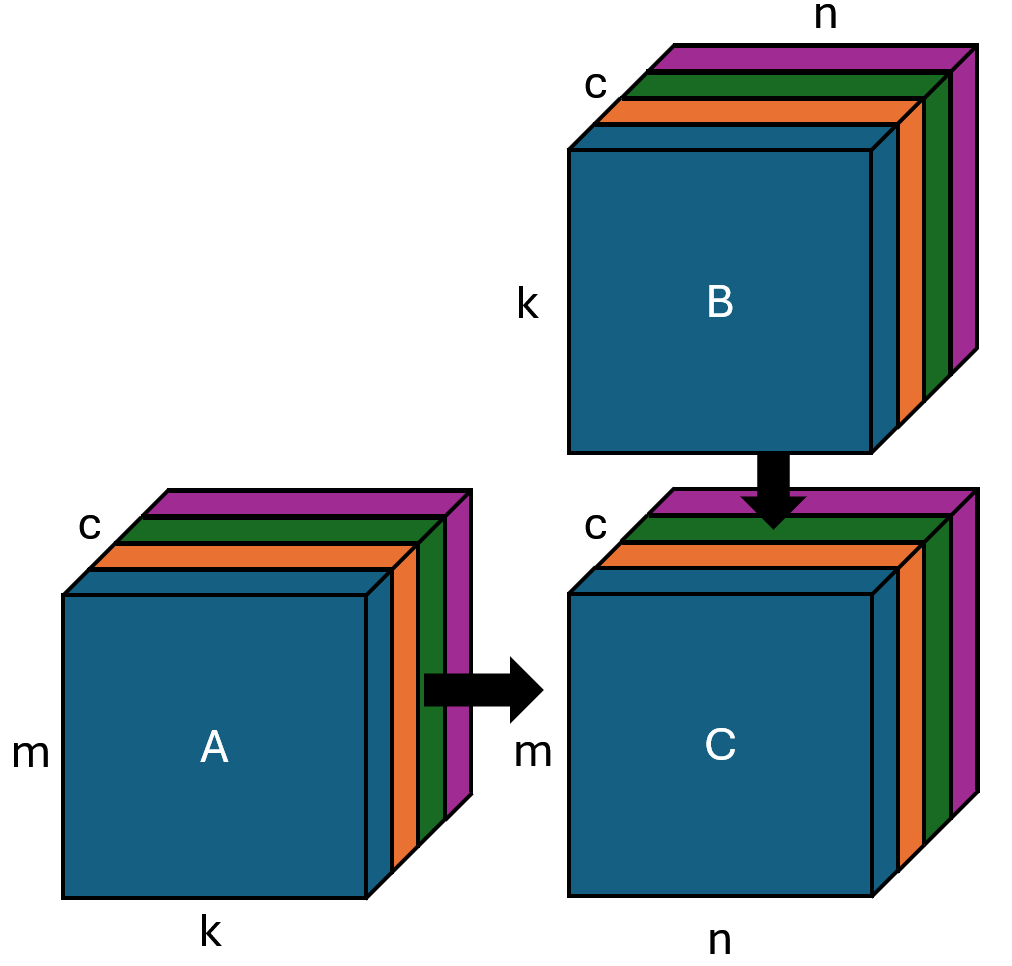
\includegraphics[width=0.3\textwidth]{dist_c.png} 
    \caption{Visualization of the Algorithm \ref{alg:c_pseudocode} for the contraction $cmk,ckn \rightarrow cmn$; 
    each color represents a process and the data they hold; 
    since the tensors are distributed along the same c dimension, each node can locally contract its chunks to generate its chunk of the output tensor.}
    \label{fig:c_algo}
    \end{figure}

\begin{algorithm}[ht]
    \begin{algorithmic}
    \Require $i = \texttt{mpi\_rank}, A_i, B_i$
    \Ensure $C_i$
    \State $A_i, B_i \rightarrow C_i$
\end{algorithmic}
\caption{Distributed c contraction}
\label{alg:c_pseudocode}
\end{algorithm}

Imagine $A$,$B$ and $C$ are distributed over a c dimension $c_0$.
As described in \ref{sec:einsum_expr} in such a case each process has to only contract its local chunks.
This algorithm is the best case since no communication has to occur and cutting a tensor among its c dimension keeps its compute intensity.

\subsection{Distributed m and n Dimensions}


\begin{figure}[ht]
    \centering
    \begin{subfigure}[t]{0.7\textwidth}
        \centering
        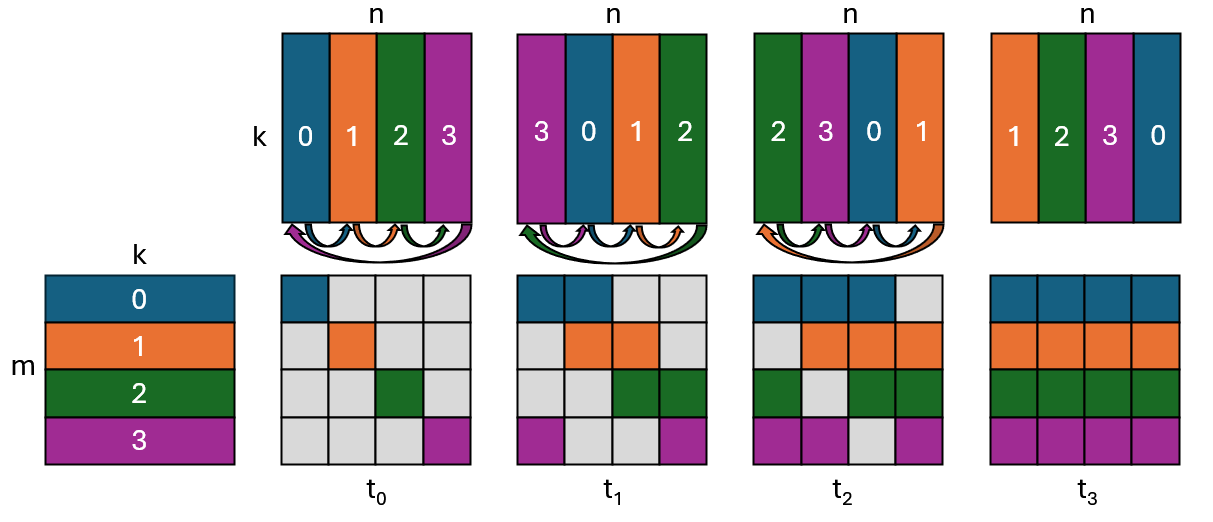
\includegraphics[width=1\textwidth]{dist_m_n.png}
        \subcaption{distributed m and n algorithm}
        \label{fig:m_n_algo_a}
    \end{subfigure}
    ~
    \begin{subfigure}[t]{0.25\textwidth}
        \centering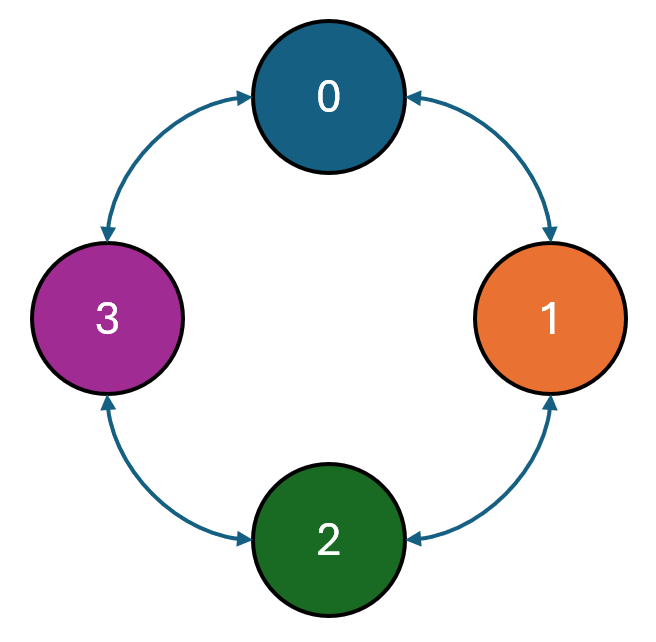
\includegraphics[width=1\textwidth]{ring.png}
        \subcaption{communication ring}
        \label{fig:m_n_algo_b}
    \end{subfigure}
    
    \caption{Visualization of Algorithm \ref{alg:m_n_pseudocode} for the contraction $mk,kn\rightarrow mn$; 
    each color represents a process and the data they hold;\\
    \ref{fig:m_n_algo_a} shows how in each step a chunk $C_{i,j}$ of the output gets calculated while the arrows show which data each process will acquire next, being coded by the arrows tip and the processes colour.\\
    \ref{fig:m_n_algo_b} shows the ring like communication setup where each process only communicates to its immediate higher and lower rank.
    }
    \label{fig:m_n_algo}
\end{figure}
    

\begin{algorithm}[ht]
        \begin{algorithmic}
        \Require $i = \texttt{mpi\_rank}, A_i, B_i$
        \Ensure $C_i$
        \State $\texttt{next} = (i+1) \mod p$
        \State $\texttt{prev} = (i+p-1) \mod p$
        \State $\texttt{comp\_buffer} \gets B_i$
        \State  $\text{for } j \text{ in } 0\dots p - 1 \text{ do:}$
        \State \indent $k \gets (i + j) \mod p$
        \State \indent \text{do in parallel:}
        \State \indent \indent $A_i, \texttt{comp\_buffer} \rightarrow C_{i,j}$
        \State \indent \indent $\texttt{mpi\_recv recv\_buffer from next}$
        \State \indent \indent $\texttt{mpi\_send comp\_buffer to prev}$
        \State \indent $\texttt{comp\_buffer} \gets \texttt{recv\_buffer}$
        \State $C_i \gets \texttt{concat}(C_{i,0}\dots C_{i,p})$
    \end{algorithmic}
    \caption{Distributed m and n contraction}
    \label{alg:m_n_pseudocode}
\end{algorithm}

Imagine $A$ and $C$ are distributed over an m dimension $m_0$ and $B$ is distributed over an n dimension $n_0$.
As described in \ref{sec:einsum_expr} we can calculate $C$ by contracting chunks $C_{i,j}$ out of $A_i$ and $B_j$ and then concatenating them over $n_0$ to end with $C$ distributed over $m_0$.
This is the first algorithm we will employ a ringlike communication scheme.
As with the master worker algorithm each process employs a dedicated communication thread.
This simply means that each process $i$ can only communicate with process $i-1$, called previous process, and process $i+1$, called next process.
Each process $i$ starts by contracting its local chunks $A_i$ and $B_i$ to calculate $C_{i,i}$.
Simultaneously each process sends its chunk $B_i$ to the previous process and receives the chunk $B_{i+1}$ from the next process.
This repeats $p$ times after which all chunks of $C_{i}$ are calculated on each process $i$ and get concatenated to $C_i$.

In the implementation we can make the final concatenation implicit as long as we contract each chunk $C_{i,j}$ already with the correct strides into the output tensor $C_i$.
Due to limitations in the binary contraction described in Section \ref{sec:einsum_ir} this is only possibly should each chunk $C_{i,j}$ be contiguous in $C_i$.
To fulfill that the implementation has to restrict the $m_0$ dimension to be the outermost dimension of $C$.

We could also consider another very similar algorithm where chunks of $A$ get sent and the final $C$ is distributed over $n_0$ instead.
Such an algorithm is omitted here, since the same effect can be achieved by swapping the input tensors as $A' \coloneqq B$ and $B' \coloneqq A$, which results in $A',B' \rightarrow C$.

The algorithm employs a ring-like communication pattern to reduce memory usage.
Instead of moving all the tensors in each time step, one could imagine an algorithm where each process keeps its chunk $B_i$ and sends them directly to each other process.
Each process still needs one tensor to contract on and another to handle the communication at the same time.
Since the initial tensor $B_i$ may no longer be moved now, this takes an additional buffer of size $|B_i|$.

\subsection{Distributed k Dimension}

\begin{figure}[ht]
    \centering
    \begin{subfigure}[t]{0.6\textwidth}
        \centering
        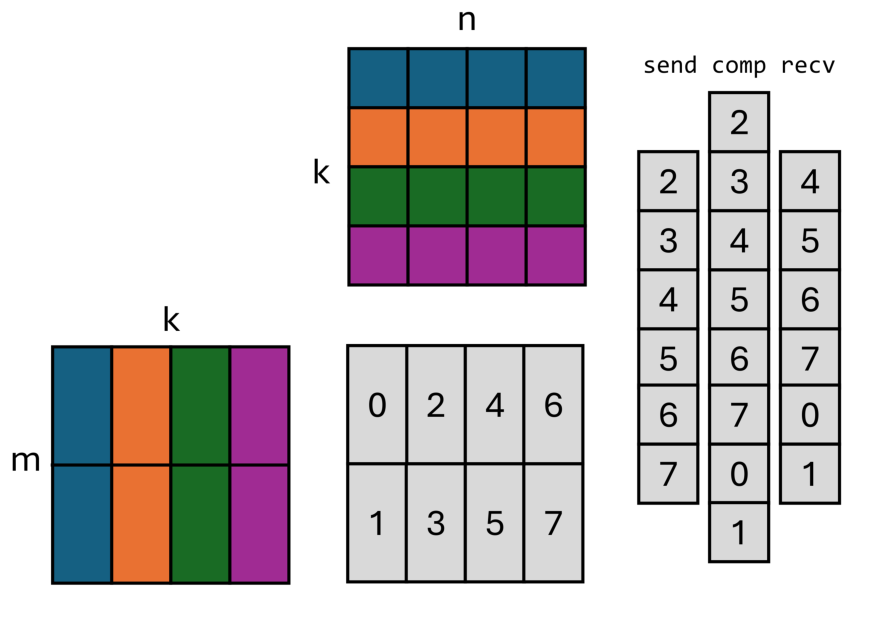
\includegraphics[width=1\textwidth]{dist_k.pdf}
        \subcaption{distributed k algorithm}
        \label{fig:k_algo_a}
    \end{subfigure}
    ~
    \begin{subfigure}[t]{0.35\textwidth}
        \centering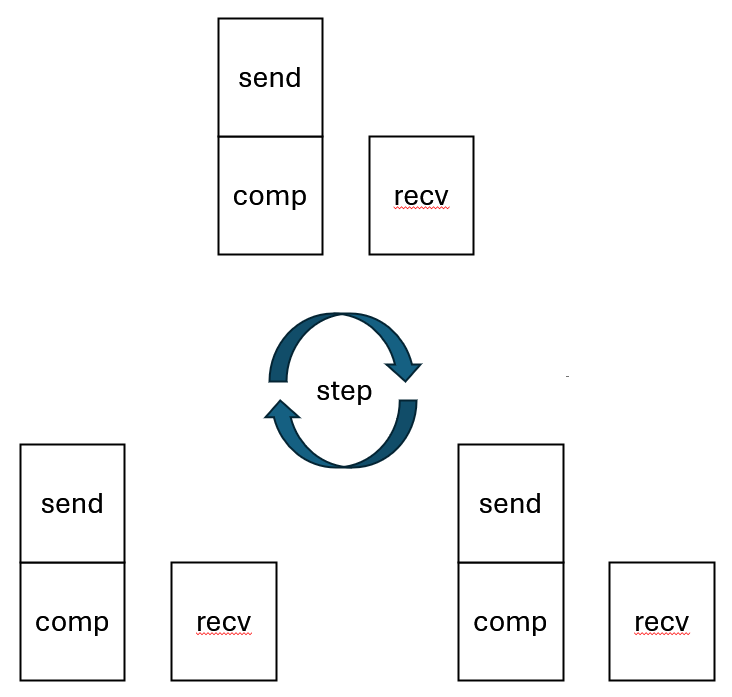
\includegraphics[width=1\textwidth]{dist_k_memory.png}
        \subcaption{rotation of buffer roles}
        \label{fig:k_algo_b}
    \end{subfigure}
    \caption{Visualization of Algorithm \ref{alg:k_pseudocode} for the contraction $mk,kn \rightarrow mn$;\\
    \ref{fig:k_algo_a} shows the order that process 0 (blue) adds its partial updates on the output chunks and which are sent to process 3 (purple) and received from process 1 (orange).\\
    \ref{fig:k_algo_b} show the output buffer as two connected buffers and the additional memory and how after each step their roles change.
    After three steps each buffer has the same role again.
    }
    \label{fig:k_algo}
\end{figure}


\begin{algorithm}[ht]
    \begin{algorithmic}
        \Require $\texttt{send\_buffer},\texttt{comp\_buffer},\texttt{recv\_buffer}$
        \Ensure $\texttt{send\_buffer},\texttt{comp\_buffer},\texttt{recv\_buffer}$
        \State $\texttt{temp} \gets {send\_buffer}$
        \State $\texttt{send\_buffer} \gets {comp\_buffer}$
        \State $\texttt{comp\_buffer} \gets {recv\_buffer}$
        \State $\texttt{recv\_buffer} \gets {temp}$
    \end{algorithmic}
    \caption{rotate}
    \label{rotate_pseudocode}
\end{algorithm}

\begin{algorithm}[ht]
    \begin{algorithmic}
    \Require $i = \texttt{mpi\_rank}, A_i, B_i, j$
    \Ensure $C_i$
    \State $\texttt{next} = (i+1) \mod p$
    \State $\texttt{prev} = (i+p-1) \mod p$
    \State $\texttt{send\_buffer} \gets \texttt{firstHalf}(C_i)$
    \State $\texttt{comp\_buffer} \gets \texttt{secondHalf}(C_i)$
    \State $\texttt{recv\_buffer} \gets \texttt{new memory}$
    \State $\text{repeat } (p+1) \mod 3 \text{ times} \texttt{ //last contraction on secondHalf}(C_i)$ 
    \State \indent $\texttt{rotate}(\texttt{send\_buffer},\texttt{comp\_buffer},\texttt{recv\_buffer})$
    \State $A_{i,0}, B_{i,next} \texttt{comp\_buffer}$
    \State  $\text{for } j \text{ in } 0\dots 2 * p - 1 \text{ do:}$
    \State \indent $ k = j \mod 2 $
    \State \indent $ m = (i + 1 + \frac{j}{2}) \mod p$
    \State \indent \text{do in parallel:}
    \State \indent \indent $A_{i,k}, B_{i,m} \rightarrow \texttt{comp\_buffer}$
    \State \indent \indent $\texttt{mpi\_recv recv\_buffer from next}$
    \State \indent \indent $\texttt{mpi\_send send\_buffer to prev}$
    \State \indent $\texttt{rotate}(\texttt{send\_buffer},\texttt{comp\_buffer},\texttt{recv\_buffer})$
    \State $A_{i,1}, B_{i,i} \rightarrow \texttt{comp\_buffer}$

\end{algorithmic}
\caption{Distributed k contraction}
\label{alg:k_pseudocode}
\end{algorithm}


Imagine $A$ and $B$ are distributed over a k dimension $k_0$, $C$ is distributed over an m dimension $m_0$ and $B$ has an n dimension $n_0$.
As described in \ref{sec:einsum_expr} each process $i$ could just compute its partial update $A_i, B_i \rightarrow C_i$ and then add them together with the other processes.
This means that each process has to hold a partial update for all values in the output tensor.
To reduce the memory footprint we augment the algorithm by calculating only chunks of the partial updates of $C$ by cutting it along $n_0$.
The basic idea is that each process gets a partial chunk from the next process, adds its own update on top and then sends the update to the previous process, employing a ring like communication scheme as shown in Figure \ref{fig:m_n_algo_b}.
If each process starts with the chunk of its next neighbour, each process ends with its own chunks of the output tensor.
To overlap computation and communication we further cut each chunk in half over $m_0$, we will call these subchunks.
This enables each process to calculate a subchunk in a step while sending the last subchunk it calculated to the previous process and get the next chunk its needs to calculate from the next process.
An example of how this would look from the perspective of process $0$ is seen in Figure \ref{fig:k_algo_a}.
We use the output chunk as memory during the algorithm to save on memory needs as seen in Figure \ref{fig:k_algo_b} as the two connected subchunks.
We still need a third subchunk so we can simultaneously send the last update, calculate the current one and receive the next one.
To ensure the updates to end in the output tensor and not in the additional memory, we will use the observation that the roles of the subchunk changes in each step in the order $\texttt{recv} \rightarrow \texttt{comp} \rightarrow \texttt{send} \rightarrow \texttt{recv}$ and that after three steps each subchunk has the same role again.
With that in mind we just need to know the end state we want, which is the bottom left one where the first subchunk of the output chunk gets calculated in the second to last step and the second subchunk gets calculated in the last one, and the number of steps, which is $2 \cdot T$.
With that information the role each subchunks starts with is just determinable by a module calculation, as seen in Algorithm \ref{alg:k_pseudocode}.

In the implementation this algorithm has additional restrictions.
Since the contraction interface only works on contiguous memory $m_0$ has to be the outermost dimension of $A$ and $C$ and $n_0$ has to be the outermost dimension of $B$.
If strided tensors are supported in the future the restriction on $n_0$ would cease to exist and as long as the additional memory is allowed to be a whole chunk instead of just a subchunk the one on $m_0$ would also be irrelevant.\\
It should also be noted that this algorithm only works under the assumption that the C tensor as input is empty, since otherwise we cannot use it during this algorithm as extra memory.
Should that be the case a slightly different algorithm would likely be preferable, where each process only calculates its own partial updates to a subchunk and then sends them as a reduction to the process which holds the output chunk in the next step.
This needs $|C|$ additional addition operations and needs a full chunk of additional memory so it can hold two subchunks at a time.

As a variation on this algorithm we could imagine an algorithm with the roles of $m_0$ and $n_0$ swapped.
This was not explored as the two inputs can be swapped for the same effect.
We could also cut $C$ and the respective input tensor over just one m or one n dimension $2 \cdot T$ times.
This would achieve the same basic algorithm and might be preferable if one dimension is much larger than the other.
